
  
  \subsection{Data Description and Preprocessing}
  
  \indent \indent
  		The dataset used for this experiment was obtained from Kaggle (a platform for predictive modelling and analytics competitions). The data set was provided by Google for a web traffic prediction competition.
		 This data file consists of  a number of views for 145063 Wikipedia pages on each day starting from 1$^{st}$ of July 2015 to 31$^{st}$ of December 2016. Each time series consists of data for the traffic generated by humans, bots or both from devices like mobile or desktop.
		 For each day, the data contains a single integer value representing the number of views that the particular Wikipedia page received on that day.  The total length of each time series is 550. There are some missing data points for some of the time series. In this experiment, we have ignored such time series for the sake of convenience. Out of 145063 time series, for this study, we have chosen the traffic generated for the  page named "2002 FIFA World Cup" on English version of Wikipedia ( i.e \url{https://en.wikipedia.org/} ) on desktop devices by all types of agents including humans and bots. \\
		 		% Some of the raw time series data chosen for this experiment are visualized in Figure \ref{fig:raw}\subref{fig:raw_12} and Figure \ref{fig:raw}\subref{fig:raw_15}.
		 
		\begin{figure}
		     \centering
		     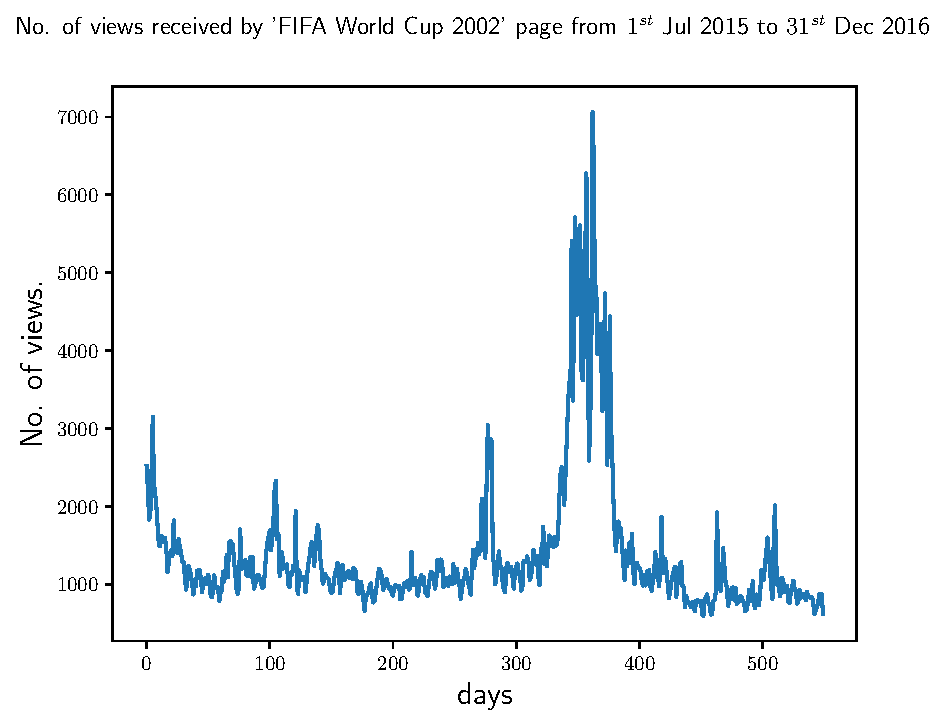
\includegraphics[width = 15cm]{./description/images/rawSignal}
			   
			   \caption{Raw data for Wikipedia Page "2002 FIFA World Cup"  which has number of views of on each date from 1$^{st}$ of July  2015 to 31$^{st}$ of December 2016. }
			\label{fig:raw}
			\end{figure}
			
For the preprocessing of the time-series used for this experiment, the following steps are followed:
\subsubsection*{\underline{Step 1}}%\label{sssec:step1}
The time series data used in this experiment has very large values ($\approx  7000$) as seen in Figure \ref{fig:raw}.  Therefore, the time-series data is non-linearly scaled down  component-wise such that the maximum value, $MAX$ of the time-series, is scaled down to the new maximum value $max$. This is done by taking small ($< < 1$) power of each component in time series $\mathbf{s}(n) = (s(1),\hdots,s(n))$. The resultant time series after the application of step 1 to the main input signal is plotted in Figure \ref{fig:preprocessingSteps}\subref{fig:squeezed}.
% The power $p$ that needs to be raised to each component of time-series is calculated using Eq. \ref{eq:power}. 
The value of $max$ can be optimized for the best performance of the network.

% \begin{equation}
% \begin{split}
% 		max &= MAX^p\\
% 		p &= log_{MAX}(max)
% \end{split}
% \label{eq:power}
% \end{equation}

  \begin{figure}
      % \centering
      \begin{subfigure}[h]{0.5\textwidth}
          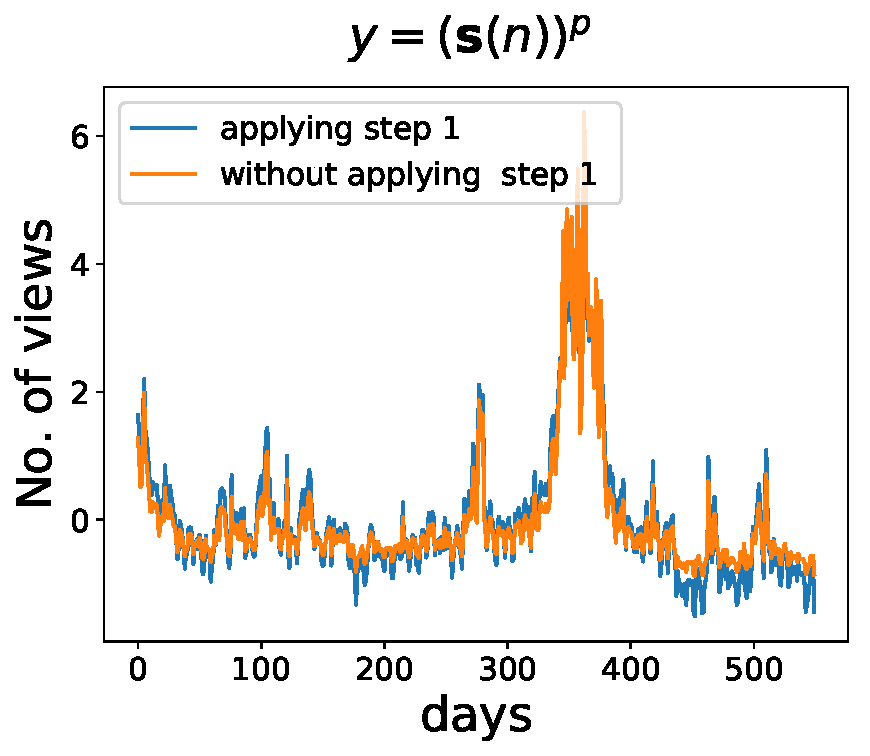
\includegraphics[width=\textwidth]{./description/images/compare_squeezed}
          \caption{ After taking component-wise power}
          \label{fig:compare_squeezed}
      \end{subfigure}
       %add desired spacing between images, e. g. ~, \quad, \qquad, \hfill etc. 
        %(or a blank line to force the subfigure onto a new line)
      \begin{subfigure}[h]{0.5\textwidth}
          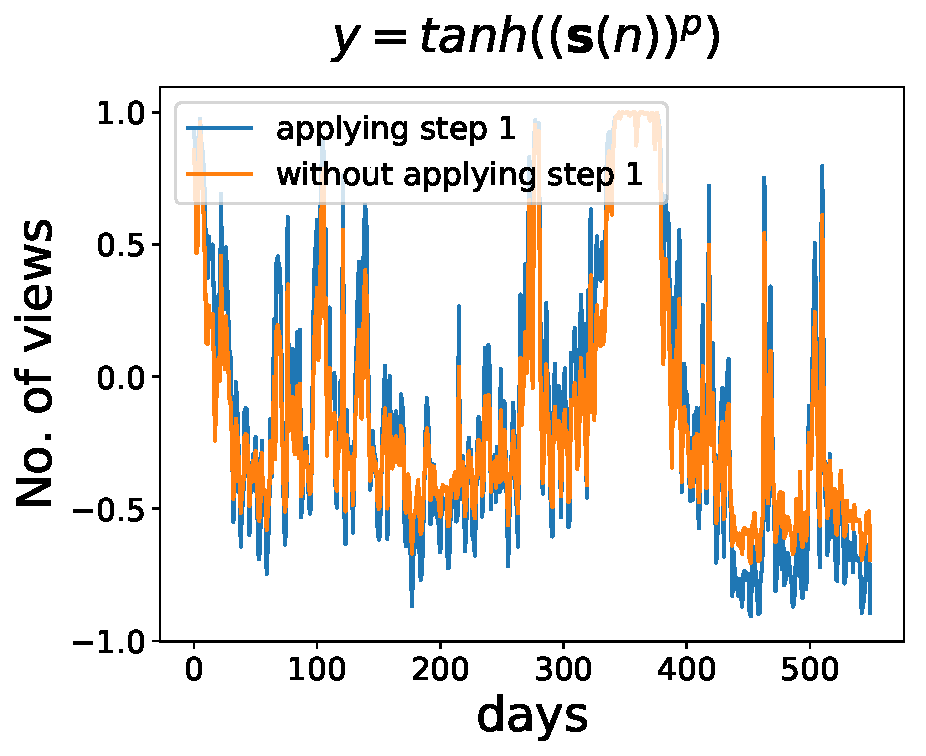
\includegraphics[width=\textwidth]{./description/images/compare_tanh}
          \caption{After further taking the $tanh$ of the signal}
          \label{fig:compare_tanh}
      \end{subfigure} 
     \begin{subfigure}[h]{0.5\textwidth}
         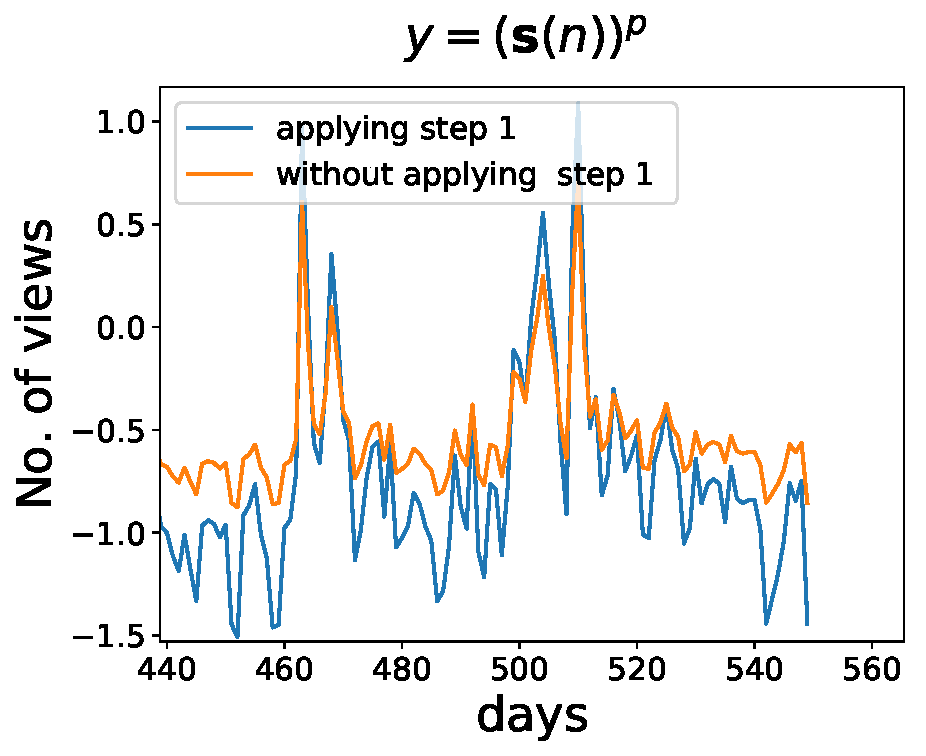
\includegraphics[width=\textwidth]{./description/images/compare_zoom_squeezed}
         \caption{ A zoomed in version of Figure \ref{fig:preprocessing}\subref{fig:compare_squeezed}.}
         \label{fig:compare_zoom_squeezed}
     \end{subfigure}
     \begin{subfigure}[h]{0.5\textwidth}
         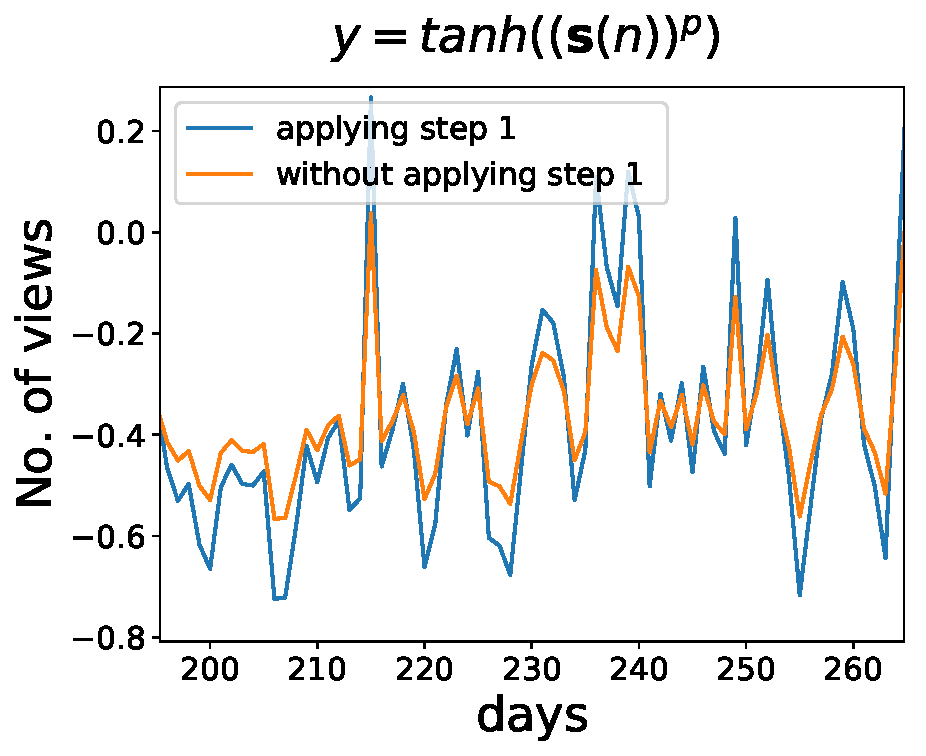
\includegraphics[width=\textwidth]{./description/images/compare_zoom_tanh}
         \caption{A zoomed in version of Figure \ref{fig:preprocessing}\subref{fig:compare_tanh}.}
         \label{fig:compare_zoom_tanh}
     \end{subfigure}
      \caption{Preprocessed time series }\label{fig:preprocessing}
  \end{figure}
  
  
\subsubsection*{\underline{Step 2}}
   The resultant time series from  step 1  is further rescaled and shifted such that it has zero mean and unit variance. The time-series data is divided componentwise by its standard deviation to make its variance unit. 
   
\subsubsection*{\underline{Step 3}}
\indent
  The resultant time series from step 2 is further applied a $tanh$ function componentwise. This strictly scales the data points in the time series in the range of $-1$ to $1$. The resultant time series after the application of step 3 to main input signal is plotted in Figure \ref{fig:preprocessingSteps}\subref{fig:tanh}.
  
  \begin{figure}[h]
      % \centering
      \begin{subfigure}[h]{0.5\textwidth}
          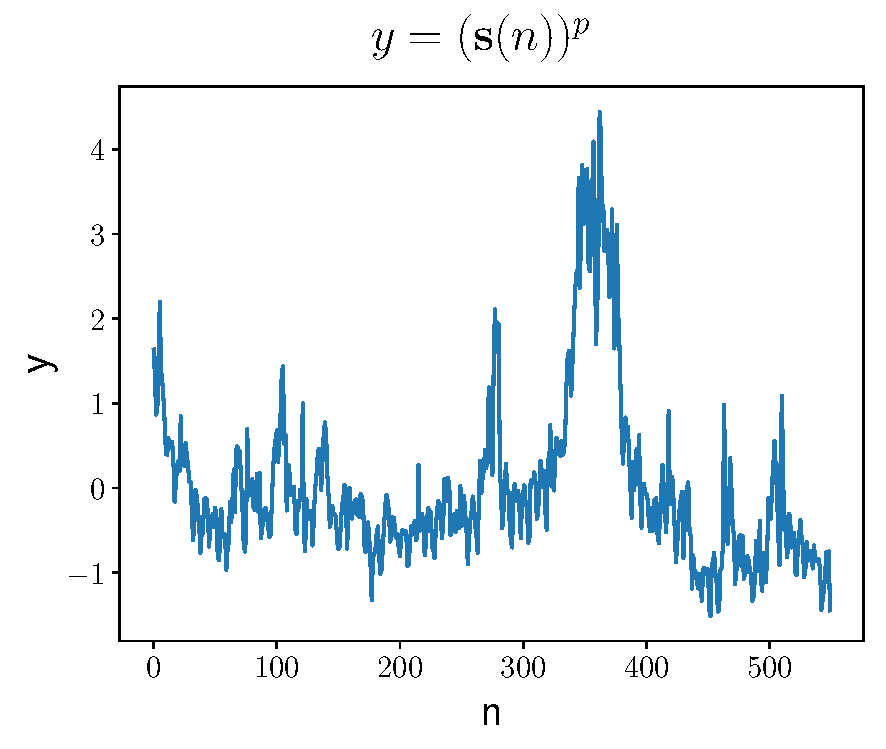
\includegraphics[width=\textwidth]{./description/images/squeezed}
          \caption{ After taking component-wise power}
          \label{fig:squeezed}
      \end{subfigure}
       %add desired spacing between images, e. g. ~, \quad, \qquad, \hfill etc. 
        %(or a blank line to force the subfigure onto a new line)
      \begin{subfigure}[h]{0.5\textwidth}
          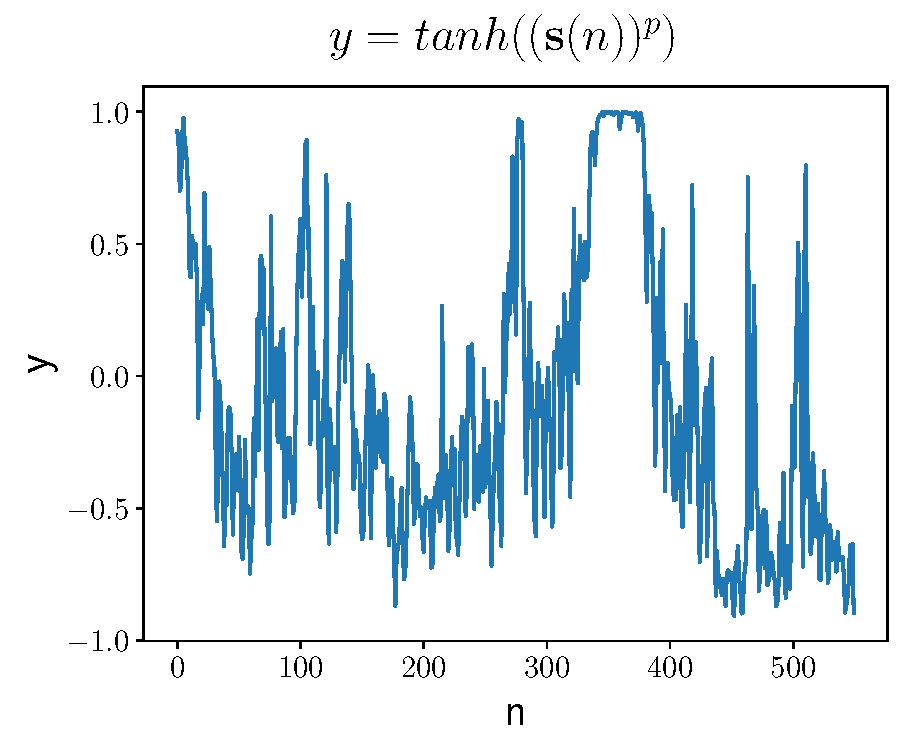
\includegraphics[width=\textwidth]{./description/images/tanh}
          \caption{After further taking the $tanh$ of the signal}
          \label{fig:tanh}
      \end{subfigure}\\
      
     
      \caption{Preprocessing steps}\label{fig:preprocessingSteps}
  \end{figure}
  
 In step 1, the higher valued data points in the signal are penalised more than the smaller ones. Therefore, the higher peaks in the input signal are shortened, and the smaller oscillations in the signal are scaled up. In  Figure  \ref{fig:preprocessing}\subref{fig:compare_squeezed} ( a zoomed in version in Figure \ref{fig:preprocessing}\subref{fig:compare_zoom_squeezed}), the orange colored signal generated with the application of only step 2 has smaller oscillations than the blue signal generated with the application of both step 1 and step 2. Even after the application of $tanh$ in step 3, the scaling up of oscillations in the blue signal generated by applying all three steps is higher than the orange colored signal that is generated without applying step 1 (see Figure \ref{fig:preprocessing} \subref{fig:compare_squeezed}, or a zoomed in version in \ref{fig:preprocessing} \subref{fig:compare_zoom_squeezed} ). Patterns become more prominent for ESN with scaling up of smaller oscillations in the input signals.  Applying $tanh$ function in step 3 further scales up the smaller oscillations in the signal and scales down the higher peaks such that the values at any time point in the signal is within the range of $-1$ to $1$.
 \subsection{Additional Input Signals}

 
 \indent \indent
 By nature, the number of views that a particular Wikipedia Page receives vary according to  days in a week and months in a year. For instance: A page related to weekend activities might receive a different proportion of views on weekends than on working days. Furthermore, Wikipedia pages on related subject matters might receive proportional number of views and could follow a similar pattern of incoming web traffic. Therefore those related input signals were added to the ESN to improvise the prediction result. In particular, we used the following approaches to find suitable additional input for the network. \\\\
 
 \begin{enumerate}
	 \item First of all, we calculate a sine wave that has the highest correlation with the main input signal. It gives the insights about the weekly pattern to the ESN.  It was further preprocessed using the same routines as used for the main input signal. This sine wave signal was further scaled with a scaling factor $sf_{sine}$ and then input to the network.
	 \item Then from the database of about 145 thousand, the top 20 time series are selected which have the highest correlation with the main input signal. The main input signal of page "2002 FIFA World Cup" on English version of Wikipedia i.e \url{https://en.wikipedia.org/} has high correlation to the pages given in Table \ref{table:addsig}. The main input signal and the mean of these additional signals after tuning it to zero mean and unit variation is plotted in Figure \ref{fig:meanvsmain}. As the additional signals are highly correlated to the main signal, these two signals have similar patterns in longer range.  These signals are further preprocessed using the same preprocessing routines as used for the main input signal. Finally, each of these additional signal is multiplied with a scaling factor $sf_{add}/NUM$, where $NUM$ is the total number of such additional inputs. To determine the correlation between any two time series we have used Pearson's correlation coefficient.\\
 	\begin{center}
 	\captionof{table}{Information about the additional signal} \label{table:addsig} 
 	\begin{tabular}{|c|c|c|} \hline
 		\textbf{Wikipedia page Title} & \textbf{Wikipedia version} & \textbf{correlation coefficient} \\ \hline
		Fußball Weltmeisterschaft 1994 & de.wikipedia.org & 0.92 \\ \hline
		2010 FIFA World Cup & en.wikipedia.org & 0.94 \\ \hline
		Copa Mundial de Fútbol de 2010 & es.wikipedia.org & 0.91 \\ \hline
		Fußball-Europameisterschaft 2008 & de.wikipedia.org & 0.90 \\ \hline
		Fußball-Europameisterschaft 1992 & de.wikipedia.org & 0.91 \\ \hline
		UEFA Euro 2008 & en.wikipedia.org &  0.91 \\ \hline
		Eurocopa 2008 & es.wikipedia.org & 0.93 \\ \hline
		2006 FIFA World Cup & en.wikipedia.org & 0.91 \\ \hline
		Fußball-Weltmeisterschaft 2010 & de.wikipedia.org & 0.92 \\ \hline
		2010 FIFA World Cup & en.wikipedia.org & 0.93 \\ \hline
		1998 FIFA World Cup & en.wikipedia.org &  0.96 \\ \hline
		Coupe du monde  de football   & fr.wikipedia.org & 0.91 \\ \hline
		Fußball-Europameisterschaft 1988 & de.wikipedia.org & 0.92 \\ \hline
		2006  FIFA World Cup & en.wikipedia.org &  0.96 \\ \hline
		\begin{otherlanguage*}{russian}
		Чемпионат мира по футболу 2002 
		\end{otherlanguage*}
		 & ru.wikipedia.org & 0.90 \\ \hline
		Fußball-Weltmeisterschaft 2002 & de.wikipedia.org &  0.93 \\ \hline
		2002 FIFA World Cup & en.wikipedia.org & 0.96 \\ \hline
		Fußball-Weltmeisterschaft 2014 & de.wikipedia.org & 0.91 \\ \hline
		2014 FIFA World Cup & en.wikipedia.org & 0.91 \\ \hline
		\begin{otherlanguage*}{russian}
		Чемпионат мира по футболу 2010 
		\end{otherlanguage*}
		& ru.wikipedia.org & 0.92 \\ \hline
		
 	\end{tabular}
 	\end{center}
	 
	 
     \begin{figure}[h]     
      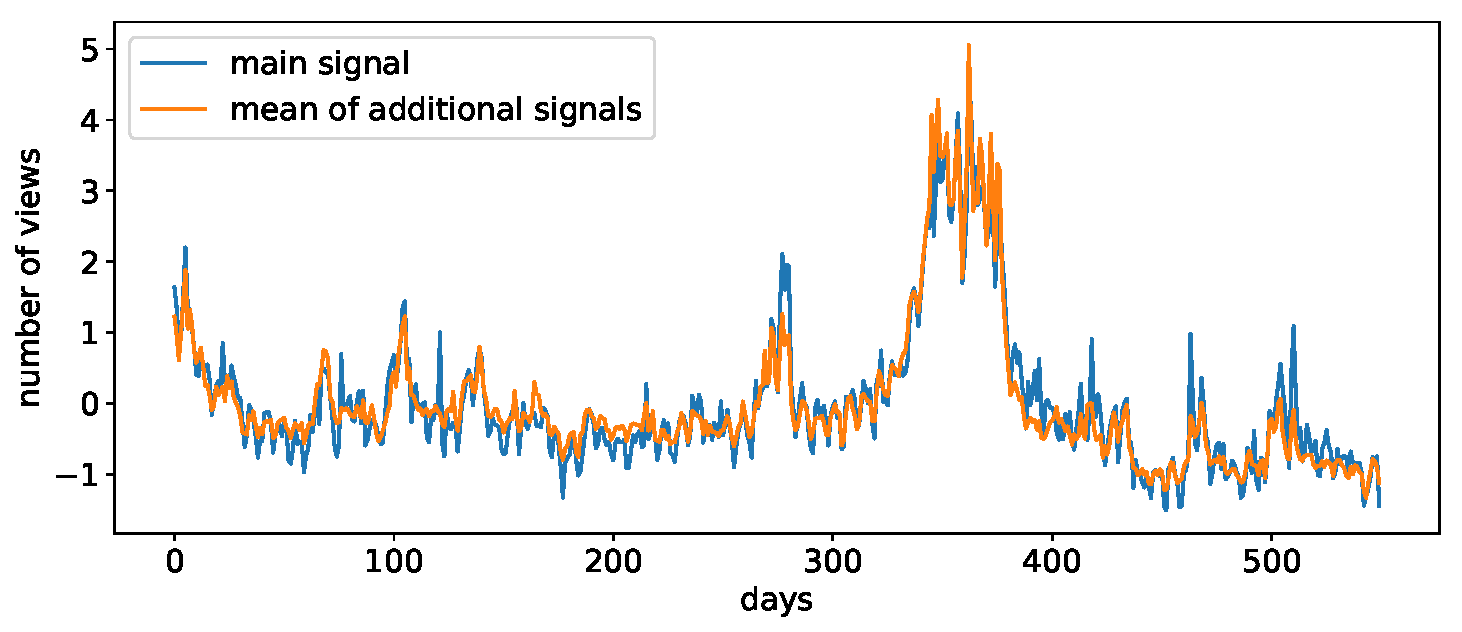
\includegraphics[width=\textwidth]{./description/images/meanvsmain}
         \caption{Main signal vs mean signal.}\label{fig:meanvsmain}
     \end{figure}
	 
	
	 
 \end{enumerate}
 
 
 
 \subsubsection{Pearson correlation coefficient}
  Pearson's correlation coefficient is the measure of the linear correlation coefficient between two time series. Its value is in the range of -1 to 1. Value close to 1 indicates that the time series are highly correlated to each other, value close -1 indicates that the time series are negatively correlated to each other and value close to 0 indicates that the two time series are unrelated. Pearson coefficient between two time series $\mathbf{X} = (x_1, \hdots, x_m)$ and $\mathbf{Y} = (y_1, \hdots, y_m)$ can be computed using the Equation \eqref{eq:pearson}.
  
  \begin{equation}
  \begin{split}
	  \rho X,Y =& \frac{cov(X,Y)}{\sigma_X \sigma_Y}\\
		=& \frac{\Sigma^{m}_{i=1}(x_i - \bar{x})(y_i - \bar{y})} {\sqrt{\Sigma^m_{i=1}(x_i - \bar{x}^2)}}
  \end{split}
   \label{eq:pearson}
  \end{equation}
  
  where:
  \begin{itemize}
	  \item $m$ is the length of time series
	  \item $x_i, y_i$ are the data points in time series $X$ and $Y$ indexed with $i$
	  \item $\bar{x_i} = \frac{1}{n}\Sigma_{i=1}^{n}x_i$  and analogously for $\bar{y}$.
	  
	  \end{itemize}
 
 




		% Max &= \text{max}\left( \mathbf{s}(n)  \right) \\
	% 	Max^p = \text{max}\left( \mathbf{s}(n)  \right) ^p\\
	% 	max &= \text{max}( (s(1),\hdots,s(n)) 
% \end{multline}
	% \begin{multiline}
% 		max = \text{max}( \mathbf{s}(n)  ^p \\
% 		max = \text{max}( (s(1),\hdots,s(n)) ^p
% 	\end{multiline}
%


\subsection{Network Setup}
\indent \indent
    
	We create a reservoir of $N = 99$ neurons. A small sized reservoir may not provide a rich set of dynamics to form the good approximation of desired signal while a large sized reservoir is computationally expensive for training. In our case, a reservoir of size in the of order of a few hundred neurons meet our demand of the prediction task. We initially used reservoir of the size of a few hundred neurons (N $\approx$ 400) and later optimized its size during cross validation phase of experiment. We have chosen the reservoir size to be multiple of 3 because later we divide the weight matrix, $\mathbf{W}$ into 9 equal regions.   %The weights of each synaptic links connecting the neurons of reservoirs are chosen randomly from uniform distribution over (-0.5, 0.5). These weights are stored in  weight matrix $\mathbf{W}\in \mathbb{R}^{N\times N}$.
	   The weights  for input links  
	 and bias vector 
	 are generated randomly from a uniform distribution over (-0.5, 0.5) and stored in matrix $\mathbf{W}^{in} \in \mathbb{R}^{N\times K}$  and $\mathbf{B} \in \mathbb{R}^{N\times 1}$ respectively. There are $K=22$ input neurons that receive 1 main input signal and each of the $21$ additional input signals and $L=31$ output neurons each of which makes $t=1,\hdots,31$ step ahead prediction.
\\
     \begin{figure}  	  
   	 
	  \begin{center}
	  \begin{tabular}{|l|r|c|}\hline
		  \
		  fast & $\approx$ 0 & =0 \\[5ex] \hline
		  $\approx$ 0 & medium & $\approx$ 0 \\[5ex] \hline
		  =0 & $\approx$ 0 & slow \\[5ex] \hline 
	  \end{tabular}	  
	  \end{center}
		\caption{Structure of weight matrix, $\mathbf{W}$.}
		 \label{fig:wmat}
	  \end{figure}
	  \\
In order to achieve a good approximation of the desired signal, the echo functions should provide a "rich" set of dynamics to combine from. The network should be prepared in a suitably "inhomogeneous" way to meet this demand. One simple method to prepare such a "rich reservoir" is to supply a network which is sparsely and randomly connected. Sparse connectivity provides for a relative decoupling of subnetworks, which encourages the development of individual dynamics \cite{shortTermMemory}. In this experiment, the network weight matrix, $\mathbf{W}$ has different weight regions to create different capability of short-term memory so that the network can capture all types of trend (slow, medium and fast trends) in the training signal. The structure of weights matrix used is presented in Figure ~\ref{fig:wmat}.\\

Values in the weight matrix for all the regions are drawn from the uniform distribution of range $-0.5$ to $0.5$ and are scaled with a scaling factor. The scaling factors for the three diagonal regions; fast, medium and slow regions, are $a, b \text{ and } c$ respectively such that $a \textgreater b \textgreater c$. For other regions, the scaling factors are almost or equal zero. These scaling factors are optimized during the training period for the better performance of the network.\\
The spectral radius of the reservoir weight matrix \textbf{W} codetermines (i) the effective time constant of the echo state network (larger spectral radius implies slower decay of impulse response) and (ii) the amount of nonlinear interaction of input components through time (larger spectral radius implies longer-range interactions) \cite{Jaeger:2007}.
  The weight matrix $\mathbf{W}_0$ is normalized to  $\mathbf{W}_1$ with its spectral radius  by putting $\mathbf{W}_1 = \left| 1/\lambda _{max}\right| \mathbf{W}_0$ where $\lambda _{max}$ is the spectral radius of $\mathbf{W}_0$. Then the weight matrix $\mathbf{W_1}$ is scaled with a scaling factor $sf_W$ such that $\mathbf{W} = sf_W \mathbf{W_1}$. Then $\mathbf{W}$ has spectral radius of $sf_W$. The choice of the spectral radius $sf_W$ of the reservoir is crucial for the eventual success of ESN training. This is because $sf_W$ is  intimately connected to the intrinsic timescale of the dynamics of the reservoir state. Small $sf_W$ lead to fast forgetting and large $sf_W$ leads to slow forgetting of the previous states.
%   means that one has a fast dynamics reservoir and large $sf_W$ (i.e close to unity) means that one has a slow reservoir. 
  Also, the input weight matrix $\mathbf{W}^{in}$  and bias vector $\mathbf{B}$ is scaled with scaling factors $sf_{Win}$ and $sf_B$ respectively. 

\subsection{Performance Metrics}\label{performance_metrics}
\indent \indent
We have used Normalized Root Mean Square Error (NRMSE) as a measure to evaluate the performance of the reservoir. NRMSE measures the difference between the predicted values $y$ and true values $r$. The values for $y$ and $r$ in this experiment are one dimensional. NRMSE for one dimensional $y$ and $r$ can be computed using the Equation \eqref{eq:nrmse}.


\begin{equation}
	NRMSE = \sqrt{\frac{\sum_{i=1}^N(y(i)-r(i))^2}{N \sigma ^2}}
\label{eq:nrmse}
\end{equation}
where $N$ denotes the number of output data points, $\sigma^2$ denotes the variance of $y$ and $r$. NRMSE with its value close to zero indicates that the quality of prediction is very good. The higher the NRMSE the lesser accurate the prediction is.


\subsection{Regularization}
In order to access the quality of the prediction produced by the training of ESN, we regularly monitor the computed output weights $\mathbf{W}^{out}$. Large weights indicate that $\mathbf{W}^{out}$ exploits and amplifies tiny differences among the dimension of  $\mathbf{x}(n)$, and can be very sensitive to deviations from the exact conditions of the trained network \cite{mantas}. To counteract this effect the regularization part $\beta \mathbf{I}$ in the ridge regression is used as mentioned in Equation  \eqref{eq:wout} .

% \subsection{Leaky Integration}
% In ordinary ESNs, the current state $\mathbf{x}(n+1)$ of the network functionally depends only on the previous state $\mathbf{x}(n)$. This property is excellent for learning discrete chaotic signals with strong oscillations but imposes difficulties when dealing with continuous slow signals. To overcome this problem, we use networks with continuous dynamics.  Networks with continuous dynamics can be approximated by updating the network with a leaky integrator. The leaking rate $\alpha$ can be intuitively seen as the value that regulates how much information about the previous state is preserved and how much information is updated by the network update function. When $\alpha$ with its value close to 0 the network state is changed very slowly since only a small ‘fraction‘ of the state is updated. On the other hand, when $\alpha$ with its value close to 1, the network state is updated very quickly. The leaking rate allows Echo State Networks to remember previous states across multiple update cycles allowing the network to learn continuous signals with long periods \cite{EchoStatesTechRep,erodriguez}.

% % The leaking rate $\alpha \in \mathbb{R}^{N\times 1}$ of the reservoir nodes can be regarded as the speed of the reservoir update dynamics discretized in time.
%  The state update  Eq. \eqref{eq:stateUpdate} is modified to Eq. \eqref{eq:stateUpdateWithLeaky}. The values


%   \begin{equation} \label{eq:stateUpdateWithLeaky}
%     \mathbf{x}(n+1) = (1-\alpha)\mathbf{x}(n) + \alpha ( f(\mathbf{Wx}(n) +  \mathbf{W}^{in}\mathbf{u}(n+1) + \mathbf{B} ) )
%   \end{equation}
 
% Each component of $\alpha \in \mathbb{R}^{N\times 1}$ can be optimized for the better performance of the network, however, this increases the number of parameters that need to be optimized, with the increase in the size of Network. Therefore to make the tuning process easier the one dimensional vector is divided into three regions so that it has three different leaking rates or scaling factors. The entire vector $\alpha$ consists and the three scaling factor are the parameters that need to be optimized.

\subsection{Cross Validation}
\indent \indent
	The length of each available time series data is $550$ out of which we leave out the last $31$ data points for the testing purpose and remaining data points are used for training purpose.\\
% 	Optimizing a parameter for a reservoir using same set of training and validation data might lead to an overfitting problem. 
% 	    An overfitted model performs well on validation set of data. However, when this overfitted model is tested on new set of testing data, its performance is very poor. Therefore, to avoid such a disaster in performance we have used a concept of cross-validation.
	\\
% The removal of some parts of the training signal for the purpose of validation results in the length of the signal to be only $519$ which poses a risk of underfitting. 
Since the length of the training part of signal is only $519$ after the removal of some part of it for the validation purpose, it poses a risk of underfitting.  By reducing the amount of data for training, there exists a risk of not capturing the important pattern/trends in the data set, which in turn increases the error induced by bias. So a cross validation scheme is required which leaves ample data for training and validation. In our case, K-fold cross validation is the first choice because it exactly satisfies the previously stated requirement.


\subsubsection{K-fold cross validation}
\label{kfold}
    
In K-fold cross validation, the available signals are split into K parts. Out of those K parts, one of them is used for validation purpose and rest K-1 split sub-signals are concatenated in the original order to form a single signal which is then used for training. This is repeated K times such that all the K splits are used exactly once as validation signal. The overall estimate  error of the cross validation, $\mathbf{CV}_k$ given by Equation \eqref{eq:crossValidaion} , is average for the error in each fold. For this experiment, we  have used $K=4$ folds.
 
 \begin{equation} \label{eq:crossValidaion}
	 \mathbf{CV}_k = \frac{1}{k} \sum^k_{i=1}{NRMSE_i}
	 \end{equation}
\subsubsection{Computational Efficiency in K-fold cross validation}
As mentioned in subsection \ref{kfold}, the input signal is divided into K splits for the cross validation and in each fold of cross validation loop, (K-1) splits are used for training and the remaining as validation signal. However this process of redoing the similar steps multiple times can be computationally redundant and expensive for longer input signals or higher values of K. Therefore, to decrease the computational cost of training the network, instead of splitting input data into K folds and performing cross validation steps, we feed the entire input signal to the state update equation \eqref{eq:stateUpdate} in a loop that runs from  $i = 1,\hdots,{n_{max}}$ ( ${n_{max}}$ is the length of the input signal). In each iteration $i$ of the loop, we  use state vector $\mathbf{x}$ of the previous iteration (i.e. at time $i-1$) which goes through a nonlinear transformation to generate state vector at time $i$. For $i = 0$,  we choose the	state vector $\mathbf{x}$ as an $N$ dimensional vector of zeros. These state vectors, $\mathbf{x}(n)$ concatenated with input, $\mathbf{u}(n)$ are stacked in state collection matrix $\mathbf{S} \in \mathbb{R}^{n_{max} \times (N+k)}$.  \\


As for ESN, before proceeding to train the network, it is necessary to remove the initial few states (eg. zero state ) which contains initial memory that is not the part of the input. Therefore first $n_0$ rows of matrix $\mathbf{S}$ are discarded. The value of $n_0$ is determined by the observations of the activations of neurons. By time $n = n_0+1$ , it is safe to assume that the effects of the arbitrary initial state have washed away and the network gives a pure reflection of the input signal \cite{jingdai}. \\

After removing the initial washout from the state collection matrix $\mathbf{S}$, it is divided into K folds. In each iteration of a loop that runs from $i=1,\hdots,K$ the input signal and teacher signal corresponding to one of the fold is used as the validation data set while the rest of the  folds and their corresponding teacher signals are used for training the network. This way we only have to compute the states using the entire signal and then reuse those computed states for training and validation during the cross validation loop. This procedure reduces the computational cost of training the network during cross validation phase.

\subsection{Computation of output weights}
\indent \indent
The learning of the output weights $\mathbf{W}^{out}$ \eqref{eq:wout} can be phrased as solving a system of linear equation
\begin{equation}
	\mathbf{W}^{out} \mathbf{S} = D
	\label{eq:linearReg}
	\end{equation}
with respect to $\mathbf{W}^{out}$. Since the goal is to minimize the quadratic error $E(\mathbf{D},\mathbf{W}^{out}\mathbf{S})$  as in \eqref{eq:nrmse}, to solve \eqref{eq:linearReg} we have used methods for finding least square solutions of overdetermined systems of linear equation i.e linear regression \cite{reservoirComputing}.\\

	 $\mathbf{W}^{out}$ is computed as the linear regression of weights of  
	    desired outputs, $\mathbf{D}$, on the harvested extended system states during the training phase, $\mathbf{S}$. We use Equation \eqref{eq:wout} to compute $\mathbf{W}^{out}$.
		



 